%%%%%%%%%%%%%%%%%%%%%%%%%%%%%%%%%%%%%%%%%%%%%%%%%%%%%%%%%%%%%%%
%% U TEXAS THESIS TEMPLATE
%
% Originally by Keith A. Gillow (gillow@maths.ox.ac.uk), 1997
% Modified by Sam Evans (sam@samuelevansresearch.org), 2007
% Modified by John McManigle (john@oxfordechoes.com), 2015
% Modified by Ulrik Lyngs (ulrik.lyngs@cs.ox.ac.uk), 2018-, for use with R Markdown
% Modified by Nilavra Bhattacharya (nilavra@utexas.edu), 2023-, for use with R Markdown
%
% Nilavra Bhattacharya, 24 Jan 2023: Following previous authors: Ulrik Lyngs and John McManigle, broad permissions are granted to use, modify, and distribute this software
% as specified in the MIT License included in this distribution's LICENSE file.
%
% Ulrik Lyngs, 25 Nov 2018: Following John McManigle, broad permissions are granted to use, modify, and distribute this software
% as specified in the MIT License included in this distribution's LICENSE file.
%
% John commented this file extensively, so read through to see how to use the various options.  Remember that in LaTeX,
% any line starting with a % is NOT executed.

%%%%% PAGE LAYOUT
% The most common choices should be below.  You can also do other things, like replace "a4paper" with "letterpaper", etc.

% 'twoside' formats for two-sided binding (ie left and right pages have mirror margins; blank pages inserted where needed):
%\documentclass[a4paper,twoside]{templates/ociamthesis}
% Specifying nothing formats for one-sided binding (ie left margin > right margin; no extra blank pages):
%\documentclass[a4paper]{ociamthesis}
% 'nobind' formats for PDF output (ie equal margins, no extra blank pages):
%\documentclass[a4paper,nobind]{templates/ociamthesis}

% As you can see from the line below, oxforddown uses the a4paper size, 
% and passes in the binding option from the YAML header in index.Rmd:
\documentclass[letterpaper, nobind]{templates/ociamthesis}


%%%%% ADDING LATEX PACKAGES
% add hyperref package with options from YAML %
\usepackage[pdfpagelabels]{hyperref}
% handle long urls
\usepackage{xurl}
% change the default coloring of links to something sensible
\usepackage{xcolor}
% single double and other spacing
\usepackage{setspace}

% for bengali fonts
% \babelprovide[import]{bangla}
% \babelfont[bangla]{rm}{kalpurush.ttf}

% \usepackage{fontspec} 
% \usepackage{polyglossia} 
% \setdefaultlanguage{english} 
% \setotherlanguages{bengali}
% \newfontfamily{\bengalifont}[Script=Bengali]{kalpurush.ttf}

% \setotherlanguages{hindi,sanskrit,bengali}
% \setmainfont{Times New Roman} 
% \newfontfamily{\devanagarifont}[Script=Devanagari]{Lohit Devanagari.ttf} 


\definecolor{mylinkcolor}{RGB}{0,0,139}
\definecolor{myurlcolor}{RGB}{0,0,139}
\definecolor{mycitecolor}{RGB}{0,33,71}

\hypersetup{
  hidelinks,
  colorlinks,
  linktocpage=true,
  linkcolor=mylinkcolor,
  urlcolor=myurlcolor,
  citecolor=mycitecolor
}


% add float package to allow manual control of figure positioning %
\usepackage{float}

% enable strikethrough
\usepackage[normalem]{ulem}

% use soul package for correction highlighting
\usepackage{color, soulutf8}
\definecolor{correctioncolor}{HTML}{CCCCFF}
\sethlcolor{correctioncolor}
\newcommand{\ctext}[3][RGB]{%
  \begingroup
  \definecolor{hlcolor}{#1}{#2}\sethlcolor{hlcolor}%
  \hl{#3}%
  \endgroup
}
% stop soul from freaking out when it sees citation commands
\soulregister\ref7
\soulregister\cite7
\soulregister\citet7
\soulregister\autocite7
\soulregister\textcite7
\soulregister\pageref7

%%%%% FIXING / ADDING THINGS THAT'S SPECIAL TO R MARKDOWN'S USE OF LATEX TEMPLATES
% pandoc puts lists in 'tightlist' command when no space between bullet points in Rmd file,
% so we add this command to the template
\providecommand{\tightlist}{%
  \setlength{\itemsep}{0pt}\setlength{\parskip}{0pt}}
 
% allow us to include code blocks in shaded environments

% User-included things with header_includes or in_header will appear here
% kableExtra packages will appear here if you use library(kableExtra)
\usepackage{booktabs}
\usepackage{longtable}
\usepackage{array}
\usepackage{multirow}
\usepackage{wrapfig}
\usepackage{float}
\usepackage{colortbl}
\usepackage{pdflscape}
\usepackage{tabu}
\usepackage{threeparttable}
\usepackage{threeparttablex}
\usepackage[normalem]{ulem}
\usepackage{makecell}
\usepackage{xcolor}


%UL set section header spacing
\usepackage{titlesec}
% 
\titlespacing\subsubsection{0pt}{24pt plus 4pt minus 2pt}{0pt plus 2pt minus 2pt}


%UL set whitespace around verbatim environments
\usepackage{etoolbox}
\makeatletter
\preto{\@verbatim}{\topsep=0pt \partopsep=0pt }
\makeatother


%%%%%%% PAGE HEADERS AND FOOTERS %%%%%%%%%
\usepackage{fancyhdr}
\setlength{\headheight}{15pt}
\fancyhf{} % clear the header and footers
\pagestyle{fancy}
\renewcommand{\chaptermark}[1]{\markboth{\thechapter. #1}{\thechapter. #1}}
\renewcommand{\sectionmark}[1]{\markright{\thesection. #1}} 
\renewcommand{\headrulewidth}{0pt}

\fancyhead[LO]{\emph{\leftmark}} 
\fancyhead[RE]{\emph{\rightmark}} 




% UL page number position 
\fancyfoot[C]{\emph{\thepage}} %regular pages
\fancypagestyle{plain}{\fancyhf{}\fancyfoot[C]{\emph{\thepage}}} %chapter pages




%%%%% SELECT YOUR DRAFT OPTIONS
% This adds a "DRAFT" footer to every normal page.  (The first page of each chapter is not a "normal" page.)
\fancyhead[R]{\emph{Draft \today}}

% IP feb 2021: option to include line numbers in PDF

% for line wrapping in code blocks
\usepackage{fancyvrb}
\usepackage{fvextra}
\DefineVerbatimEnvironment{Highlighting}{Verbatim}{breaklines=true, breakanywhere=true, commandchars=\\\{\}}

% This highlights (in blue) corrections marked with (for words) \mccorrect{blah} or (for whole
% paragraphs) \begin{mccorrection} . . . \end{mccorrection}.  This can be useful for sending a PDF of
% your corrected thesis to your examiners for review.  Turn it off, and the blue disappears.
\correctionstrue


%%%%% BIBLIOGRAPHY SETUP
% Note that your bibliography will require some tweaking depending on your department, preferred format, etc.
% If you've not used LaTeX before, I recommend just using pandoc for citations -- this is what's used unless you specific e.g. "citation_package: natbib" in index.Rmd
% If you're already a LaTeX pro and are used to natbib or something, modify as necessary.

% this allows the latex template to handle pandoc citations
\newlength{\cslhangindent}
\setlength{\cslhangindent}{1.5em}
\newlength{\csllabelwidth}
\setlength{\csllabelwidth}{3em}
\newlength{\cslentryspacingunit} % times entry-spacing
\setlength{\cslentryspacingunit}{\parskip}
\newenvironment{CSLReferences}[2] % #1 hanging-ident, #2 entry spacing
 {% don't indent paragraphs
  \setlength{\parindent}{0pt}
  % turn on hanging indent if param 1 is 1
  \ifodd #1
  \let\oldpar\par
  \def\par{\hangindent=\cslhangindent\oldpar}
  \fi
  % set entry spacing
  \setlength{\parskip}{1mm}
  \setlength{\baselineskip}{6mm}
 }%
 {}
\usepackage{calc}
\newcommand{\CSLBlock}[1]{#1\hfill\break}
\newcommand{\CSLLeftMargin}[1]{\parbox[t]{\csllabelwidth}{#1}}
\newcommand{\CSLRightInline}[1]{\parbox[t]{\linewidth - \csllabelwidth}{#1}\break}
\newcommand{\CSLIndent}[1]{\hspace{\cslhangindent}#1}




% Uncomment this if you want equation numbers per section (2.3.12), instead of per chapter (2.18):
%\numberwithin{equation}{subsection}


%%%%% THESIS / TITLE PAGE INFORMATION
% Everybody needs to complete the following:
\title{LongSAL: A Longitudinal Search as Learning Study With University Students}
\author{Nilavra Bhattacharya}


% Master's candidates who require the alternate title page (with candidate number and word count)
% must also un-comment and complete the following three lines:

% Uncomment the following line if your degree also includes exams (eg most masters):
%\renewcommand{\submittedtext}{Submitted in partial completion of the}
% Your full degree name.  (But remember that DPhils aren't "in" anything.  They're just DPhils.)
\degree{Doctor of Philosophy}

% Term and year of submission, or date if your board requires (eg most masters)



%%%%% YOUR OWN PERSONAL MACROS
% This is a good place to dump your own LaTeX macros as they come up.

% To make text superscripts shortcuts
\renewcommand{\th}{\textsuperscript{th}} % ex: I won 4\th place
\newcommand{\nd}{\textsuperscript{nd}}
\renewcommand{\st}{\textsuperscript{st}}
\newcommand{\rd}{\textsuperscript{rd}}

%%%%% THE ACTUAL DOCUMENT STARTS HERE
\begin{document}

%%%%% CHOOSE YOUR LINE SPACING HERE
% This is the official option.  Use it for your submission copy and library copy:
\setlength{\textbaselineskip}{22pt plus2pt}
% This is closer spacing (about 1.5-spaced) that you might prefer for your personal copies:
%\setlength{\textbaselineskip}{18pt plus2pt minus1pt}

% You can set the spacing here for the roman-numbered pages (acknowledgements, table of contents, etc.)
\setlength{\frontmatterbaselineskip}{17pt plus1pt minus1pt}

% UL: You can set the line and paragraph spacing here for the separate abstract page to be handed in to Examination schools
\setlength{\abstractseparatelineskip}{13pt plus1pt minus1pt}
\setlength{\abstractseparateparskip}{0pt plus 1pt}

% UL: You can set the general paragraph spacing here - I've set it to 2pt (was 0) so
% it's less claustrophobic
\setlength{\parskip}{2pt plus 1pt}

%
% Customise title page
%
\def\crest{}
\renewcommand{\university}{The University of Texas at Austin}
\renewcommand{\submittedtext}{}
\renewcommand{\thesistitlesize}{\fontsize{22pt}{28pt}\selectfont}
\renewcommand{\gapbeforecrest}{25mm}
\renewcommand{\gapaftercrest}{25mm
}


% Leave this line alone; it gets things started for the real document.
\setlength{\baselineskip}{\textbaselineskip}


%%%%% CHOOSE YOUR SECTION NUMBERING DEPTH HERE
% You have two choices.  First, how far down are sections numbered?  (Below that, they're named but
% don't get numbers.)  Second, what level of section appears in the table of contents?  These don't have
% to match: you can have numbered sections that don't show up in the ToC, or unnumbered sections that
% do.  Throughout, 0 = chapter; 1 = section; 2 = subsection; 3 = subsubsection, 4 = paragraph...

% The level that gets a number:
\setcounter{secnumdepth}{4}
% The level that shows up in the ToC:
\setcounter{tocdepth}{4}


%%%%% ABSTRACT SEPARATE
% This is used to create the separate, one-page abstract that you are required to hand into the Exam
% Schools.  You can comment it out to generate a PDF for printing or whatnot.

% JEM: Pages are roman numbered from here, though page numbers are invisible until ToC.  This is in
% keeping with most typesetting conventions.
\begin{romanpages}

% Title page is created here
% original code:
% \maketitle

% --------- start: UTexas Frontmatter (committee membership, title page) -------

% ~~~~ committee membership page ~~~~
% \thispagestyle{empty}
\begin{center}
  The Dissertation Committee for Nilavra Bhattacharya\\
  certifies that this is the approved version of the following Dissertation:\\
  \vspace*{30pt}
  \begin{spacing}{2}
    {\Large{\textbf{LongSAL: A Longitudinal Search as Learning Study With University Students}}}
  \end{spacing}
\end{center}

\vspace*{55pt}

\phantom{x}\hspace{45ex} {\large{\textbf{Committee:}}}\\
% \vspace*{12pt}

\begin{flushright}
  Jacek Gwizdka, Supervisor\\
  \vspace*{24pt}
  Soo-Young Rieh\\
  \vspace*{24pt}
  Matthew Lease\\
  \vspace*{24pt}
  Robert Capra
\end{flushright}


% ~~~~ title page ~~~~
\newpage
% \thispagestyle{empty}
\begin{center}
  
  \begin{spacing}{2}
    {\Large{\textbf{LongSAL: A Longitudinal Search as Learning Study With University Students}}}
  \end{spacing}
  
  \vspace*{24pt}

  \begin{spacing}{1.4}
    by\\
    
    \vspace*{24pt}
    
    {\Large{\textbf{Nilavra Bhattacharya নীলাভ্র ভট্টাচার্য্য}}}\\
    
    \vspace*{72pt}
    
    {\Large{\textbf{Dissertation}}}\\
    
    \vspace*{24pt}
    
    Presented to the Faculty of the Graduate School of\\
    The University of Texas at Austin\\
    in Partial Fulfillment\\
    of the Requirements\\
    for the Degree of\\
    
    \vspace*{30pt}
    
    {\Large{\textbf{Doctor of Philosophy}}}\\
    
    \vfill

    {\large{The University of Texas at Austin\\
    May 2023}}

  \end{spacing}
\end{center}


% --------- end: UTexas Frontmatter (committee membership, title page) -------


%%%%% DEDICATION

%%%%% ACKNOWLEDGEMENTS


\begin{acknowledgements}
 	This section will be fleshed out in more detail after the initial committee-submission on Feb 27, 2023.
 For now, I wish to thank the following people :

 \begin{itemize}
 \tightlist
 \item
   Committee Members: Jacek Gwizdka, Soo Young Rieh, Matt Lease, Rob Capra
 \end{itemize}
\end{acknowledgements}



%%%%% ABSTRACT


% ----------- original abstract ----------
% \renewcommand{\abstracttitle}{Abstract}
% \begin{abstract}
% 	Learning today is about navigation, discernment, induction, and synthesis of the wide body of information on the Internet present ubiquitously at every student's fingertips. Learning, or addressing a gap in one's knowledge, has been well established as an important motivator behind information-seeking activities. The Search as Learning research community advocates that online information search systems should be reconfigured to become educational platforms to foster learning and sensemaking. Modern search systems have yet to adapt to support this function. An important step to foster learning during online search is to identify behavioural patterns that distinguish searchers gaining more vs.~less knowledge during search. Previous efforts have primarily studied searchers in the short term, typically during a single lab session. Many researchers have expressed their concern over this ephemeral approach, as learning takes place over time, and is not fleeting. We propose an exploratory longitudinal study to analyze the long-term searching behaviour of students enrolled in a university course, over the span of a university semester. Our research aims are to identify if and how students' searching behaviour changes over time, as they gain new knowledge on a subject; and how do processes like motivation, metacognition, self-regulation, and other individual differences moderate their `searching as learning' behaviour. Findings from this exploratory longitudinal study will help to build improved search systems that foster human learning and sensemaking, and are more equitable in the face of learner diversity.
% \end{abstract}

% --------- start: UTexas abstract -------
\begin{center}
  \textbf{Abstract}\\
  
  \vspace{18pt}
  
  \begin{spacing}{2}
    {\Large{\textbf{LongSAL: A Longitudinal Search as Learning Study With University Students}}}
  \end{spacing}

  \vspace{18pt}

  \begin{spacing}{1.4}
    Nilavra Bhattacharya নীলাভ্র ভট্টাচার্য্য, PhD TBD\\
    The University of Texas at Austin, 2023\\
    \vspace{24pt}
    Supervisor: Jacek Gwizdka
  \end{spacing}

\end{center}

\begin{spacing}{1.5}
  \indent
  % \indent
  Learning today is about navigation, discernment, induction, and synthesis of the wide body of information on the Internet present ubiquitously at every student's fingertips. Learning, or addressing a gap in one's knowledge, has been well established as an important motivator behind information-seeking activities. The Search as Learning research community advocates that online information search systems should be reconfigured to become educational platforms to foster learning and sensemaking. Modern search systems have yet to adapt to support this function. An important step to foster learning during online search is to identify behavioural patterns that distinguish searchers gaining more vs.~less knowledge during search. Previous efforts have primarily studied searchers in the short term, typically during a single lab session. Many researchers have expressed their concern over this ephemeral approach, as learning takes place over time, and is not fleeting. We propose an exploratory longitudinal study to analyze the long-term searching behaviour of students enrolled in a university course, over the span of a university semester. Our research aims are to identify if and how students' searching behaviour changes over time, as they gain new knowledge on a subject; and how do processes like motivation, metacognition, self-regulation, and other individual differences moderate their `searching as learning' behaviour. Findings from this exploratory longitudinal study will help to build improved search systems that foster human learning and sensemaking, and are more equitable in the face of learner diversity.
\end{spacing}

% --------- end: UTexas abstract -------



%%%%% MINI TABLES
% This lays the groundwork for per-chapter, mini tables of contents.  Comment the following line
% (and remove \minitoc from the chapter files) if you don't want this.  Un-comment either of the
% next two lines if you want a per-chapter list of figures or tables.
\dominitoc % include a mini table of contents

% This aligns the bottom of the text of each page.  It generally makes things look better.
\flushbottom

% This is where the whole-document ToC appears:
\tableofcontents

\listoffigures
	\mtcaddchapter
  	% \mtcaddchapter is needed when adding a non-chapter (but chapter-like) entity to avoid confusing minitoc

% Uncomment to generate a list of tables:
\listoftables
  \mtcaddchapter
%%%%% LIST OF ABBREVIATIONS
% This example includes a list of abbreviations.  Look at text/abbreviations.tex to see how that file is
% formatted.  The template can handle any kind of list though, so this might be a good place for a
% glossary, etc.

% The Roman pages, like the Roman Empire, must come to its inevitable close.
\end{romanpages}

%%%%% CHAPTERS
% Add or remove any chapters you'd like here, by file name (excluding '.tex'):
\flushbottom

% all your chapters and appendices will appear here
\hypertarget{introduction}{%
\chapter{Introduction}\label{introduction}}

\hypertarget{sec_intro_overview}{%
\section{Searching as Learning: Overview}\label{sec_intro_overview}}

Searching for information is a fundamental human activity.
In the modern world, it is frequently conducted by users interacting with online
search systems (e.g., web search engines), or more formally,
\textbf{Information Retrieval} (IR) systems. As early as in 1980, Bertam
Brookes, in his `fundamental equation' of information and knowledge, had
stated that an information searcher's current state of knowledge is
changed to a new knowledge structure by exposure to information
(\protect\hyperlink{ref-brookes1980foundations}{Brookes, 1980, p. 131}). This indicates that searchers acquire
new knowledge in the search process, and the same information will have
different effects on different searchers' knowledge states. Fifteen
years later, (\protect\hyperlink{ref-marchionini1995information}{Marchionini, 1995}) described information seeking
as ``a process, in which humans purposefully engage in order to change
their state of knowledge''. Thus, we have known for quite a while that
search is driven by higher-level human needs, and IR systems are a means
to an end, and not the end in itself. \textbf{Interactive information
retrieval} (IIR), a.k.a. human-computer information retrieval (HCIR)
(\protect\hyperlink{ref-marchionini2006toward}{Marchionini, 2006}) refers to the study and evaluation of users'
interaction with IR systems and users' satisfaction with the retrieved
information (\protect\hyperlink{ref-borlund2013interactive}{Borlund, 2013}).

Despite their technological marvels, modern IR systems falls short in
several aspects of fully satisfying the higher level human need for
information. In essence, IR systems are software that take, as input,
some query, and return as output some ranked list of resources.

\begin{quote}
~~~~~~~Within the context of information seeking, (search engines and IR systems) \textbf{feel} like they play a prominent role in our lives, when in actuality, they only play a small role: the \textbf{retrieval} part of information \ldots{}

\begin{itemize}
\item
  Search engines \textbf{don't help us identify what we need} -- that's up to us; search engines don't question what we ask for, though they do recommend queries that use similar words.
\item
  Search engines \textbf{don't help us choose a source} -- though they are themselves a source, and a heavily marketed one, so we are certainly compelled to choose search engines over other sources, even when other sources might have better information.
\item
  Search engines \textbf{don't help us express our query} accurately or precisely -- though they will help with minor spelling corrections.
\item
  Search engines do help retrieve information---this is the primary part that they automate.
\item
  Search engines \textbf{don't help us evaluate the answers we retrieve} --
  it's up to us to decide whether the results are relevant, credible,
  true; Google doesn't view those as their responsibility.
\item
  Search engines \textbf{don't help us sensemake} -- we have to use our
  minds to integrate what we've found into our knowledge.
\end{itemize}

-- (\protect\hyperlink{ref-ko2021seeking}{Ko, 2021})
\end{quote}

In recent years, the IIR research community has been actively promoting
the \textbf{Search as Learning} (SAL) research direction. This fast-growing
community of researchers propose that search environments should be
augmented and reconfigured to foster learning, sensemaking, and
long-term knowledge-gain. Various workshops and seminars have been
organized to develop research agendas at the interaction of IIR and the
Learning Sciences
(\protect\hyperlink{ref-agosti2014evaluation}{Agosti et al., 2014}; \protect\hyperlink{ref-allan2012frontiers}{Allan et al., 2012}; \protect\hyperlink{ref-collins2017search}{Collins-Thompson et al., 2017}; \protect\hyperlink{ref-freund2013searching}{Freund et al., 2013}, \protect\hyperlink{ref-freund2014searching}{2014}; \protect\hyperlink{ref-gwizdka2016search}{Gwizdka et al., 2016})
Additionally, special issues on Search as Learning have also been
published in the \emph{Journal of Information Science} (\protect\hyperlink{ref-hansen2016editorial}{Hansen \& Rieh, 2016})
and in the \emph{Information Retrieval Journal} (\protect\hyperlink{ref-eickhoff2017introduction}{Eickhoff et al., 2017}).
Articles in these special issued presented landmark literature reviews
(\protect\hyperlink{ref-rieh2016searching}{Rieh et al., 2016}; \protect\hyperlink{ref-vakkari2016searching}{Vakkari, 2016}), research agendas, and ideas
in this direction. Overall, these works generally advocate that future
research in this domain should aim to:

\begin{itemize}
\item
  understand the contexts in which people search to learn
\item
  understand factors that can influence learning outcomes
\item
  understand how search behaviours can predict learning outcomes
\item
  develop search systems to better support learning and sensemaking
\item
  help searchers be more critical consumers of information
\item
  understand the cognitive biases fostered by existing search systems
\item
  develop search engine ranking algorithms and interface tools that
  foster long term knowledge gain
\end{itemize}

Parallelly, the Educational Science and the Learning Science research
communities have also been organizing workshops and formulating research
agendas to conceptualize forms of `new learning'
(\protect\hyperlink{ref-cope2013new}{Cope \& Kalantzis, 2013}; \protect\hyperlink{ref-kalantzis2012newa}{Kalantzis \& Cope, 2012}; \protect\hyperlink{ref-newlondon1996pedagogy}{New London Group, 1996}) that are
afforded by innovations in digital technologies and e-learning ecologies
(\protect\hyperlink{ref-cope2017elearningc}{Cope \& Kalantzis, 2017}). Higher education researchers have been
increasingly studying how students' information search and information
use behaviour affect and support their learning
(\protect\hyperlink{ref-weber2019informationseeking}{Weber et al., 2019}, \protect\hyperlink{ref-weber2018can}{2018}; \protect\hyperlink{ref-zlatkin2021students}{Zlatkin-Troitschanskaia et al., 2021}).
Efforts are underway to conceptualize a theoretical framework around new
forms of e-Learning that is aided and afforded by digital technologies
(\protect\hyperlink{ref-amina2017active}{Amina, 2017}; \protect\hyperlink{ref-cope2017elearningc}{Cope \& Kalantzis, 2017}). In the community's own words:
``learning today is more about navigation, discernment, induction, and
synthesis'' of the wide body of information present ubiquitously at every
student's fingertips (\protect\hyperlink{ref-amina2017active}{Amina, 2017}). Therefore, ``knowing the source,
finding the source, and using the information aptly is important to
learn and know now more than ever before'' (\protect\hyperlink{ref-cope2013new}{Cope \& Kalantzis, 2013}). All of these
interests in the intersection of searching and learning goes to
emphasize that understanding learning during search is critical to
improve human-information interaction.

\hypertarget{sec_intro_problem_statement}{%
\section{Problem Statement}\label{sec_intro_problem_statement}}

A major limitation in the area of Search as Learning, Interactive IR
(IIR), and more broadly, in Human-Computer Interaction (HCI) research is
that, the user is examined in the short-term, typically over the course
of a single experimental session in a lab
(\protect\hyperlink{ref-karapanos2021advances}{Karapanos et al., 2021}; \protect\hyperlink{ref-kelly2009evaluation}{Kelly et al., 2009}; \protect\hyperlink{ref-HCIUXres81_online}{Koeman, 2020}; \protect\hyperlink{ref-zlatkin2021students}{Zlatkin-Troitschanskaia et al., 2021}).
Very few studies exist in the search-as-learning domain that have
observed \emph{the same participant} over a longer period of time than a
single search session
(\protect\hyperlink{ref-kelly2006measuring_a}{Kelly, 2006a}, \protect\hyperlink{ref-kelly2006measuring_b}{2006b}; \protect\hyperlink{ref-kuhlthau2004seeking}{Kuhlthau, 2004}; \protect\hyperlink{ref-vakkari2001changes}{Vakkari, 2001}; \protect\hyperlink{ref-white2009characterizing}{White et al., 2009}; \protect\hyperlink{ref-wildemuth2004effects}{Wildemuth, 2004}).
This ephemeral approach has acute implications in any domain where
learning is involved because ``learning is a \emph{process} that leads to
\emph{change} in knowledge \ldots{} (which) unfolds over time'' (\protect\hyperlink{ref-ambrose2010howa}{Ambrose et al., 2010}),
and ``\ldots does not happen all at once''(\protect\hyperlink{ref-white_2016_iwss_learning}{White, 2016b}).

\textbf{To the best of the author's knowledge, almost no new longitudinal
studies were reported in major search-as-learning literature in the last
five years, that systematically studied students' information search
behaviour and information-use over the long term, in their \emph{in-situ}
naturalistic environment and contexts, and linked those behaviours
quantitatively to the students' learning outcomes and individual
differences.}

Higher education students are increasingly using the
Internet as their main learning environment and source of information
when studying. Yet, the short term nature of research in this domain
creates significant gaps in our knowledge regarding how students'
information search behaviour and information use develop over time, and
how it affects their learning (\protect\hyperlink{ref-zlatkin2021students}{Zlatkin-Troitschanskaia et al., 2021}).

\begin{quote}
\emph{When research in this area ``relies so heavily on (short-term) lab studies, can we
realistically say we are comprehensively studying human-tech
interactions -- when many of those interactions take place over long
periods of time in real-world contexts? \ldots{} An over-reliance on short
studies risks inaccurate findings, potentially resulting in prematurely
embracing or disregarding new concepts.''}

-- (\protect\hyperlink{ref-HCIUXres81_online}{Koeman, 2020}).
\end{quote}

Current search engines and information retrieval systems ``do not help us
know what we want to know, \ldots do not help us know if what we've found is
relevant or true; and they do not help us make sense of the retrieved
information. All they do is quickly retrieve what other people on the
internet have shared'' (\protect\hyperlink{ref-ko2021seeking}{Ko, 2021}). Unless we have more long-term
understanding of the nature of knowledge gain during search, the
limitations of current search systems will continue to persist.
Increased knowledge and understanding of students', and more broadly
searchers', information searching and learning behaviour over time will
help us to overcome the limitations of current IR systems, and transform
them into rich learning spaces where ``search experiences and learning
experiences are intertwined and even synergized'' (\protect\hyperlink{ref-url_rieh_homepage}{Rieh, 2020}).
The internet and digital educational technologies offer great
opportunities to transform learning and the education experience.
Enabled by our increased comprehension of the longitudinal
searching-as-learning process, improved and validated by empirical data,
we can create a new wave of fundamentally transformative educational
technologies and ``e-learning ecologies, that will be more engaging for
learners, more effective (than traditional classroom practices), more
resource efficient, and more equitable in the face of learner diversity''
(\protect\hyperlink{ref-cope2017elearningc}{Cope \& Kalantzis, 2017}).

\hypertarget{sec_intro_purpose}{%
\section{Purpose of this Dissertation Proposal}\label{sec_intro_purpose}}

To address the gaps in our knowledge of how information searching
influences students' learning process over time, this dissertation
proposal proposes to conduct a semester-long longitudinal study (approx.
16 weeks) with university student participants. The overarching research
aim is to identify how students' online searching behaviour correlate
with their learning outcomes for a particular university course.
Building upon principles from the Learning Sciences
(\protect\hyperlink{ref-ambrose2010howa}{Ambrose et al., 2010}; \protect\hyperlink{ref-council2000how}{National Research Council, 2000}; \protect\hyperlink{ref-novak2010learninga}{Novak, 2010}; \protect\hyperlink{ref-sawyer2005cambridge}{Sawyer, 2005}),
and empirical evidences from the Information Sciences
(\protect\hyperlink{ref-rieh2016searching}{Rieh et al., 2016}; \protect\hyperlink{ref-vakkari2016searching}{Vakkari, 2016}; \protect\hyperlink{ref-white2016interactions}{White, 2016a}),
this dissertation proposal aims to

\begin{itemize}
\tightlist
\item
  situate students as learners in their naturalistic contexts, and
  characterized by their individual differences,
\item
  measure students' information search and information use behaviour
  over time, and
\item
  correlate the information search behaviour with the learning
  outcomes for the university course.
\end{itemize}

Learning, or addressing a gap in one's knowledge, has been well
established as an important motivator behind information-seeking
activities (Section \protect\hyperlink{sec_intro_overview}{1.1}). Therefore, search systems that support
rapid learning across a number of searchers, and a range of tasks, can
be considered as more effective search systems (\protect\hyperlink{ref-white2016interactions}{White, 2016a, p. 310}). This dissertation proposal takes a step in this direction. ``It
opens great expectations for many-sided, great contribution to our
knowledge on the relations between search process and learning outcomes''
(\protect\hyperlink{ref-bhattacharya2021longitudinal}{Bhattacharya, 2021} anonymous reviewer).

\hypertarget{sec_intro_outline}{%
\section{Outline}\label{sec_intro_outline}}

This dissertation proposal document is structured as follows. First,
principles of learning and relevant background from the domain of
Educational Sciences are presented in Chapter 2. Next, relevant
empirical evidences from the Information Searching Literature are
discussed in Chapter 3. Chapter 4 presents the research questions, the
overarching hypotheses, and discusses their rationale in the context of
the existing research gaps. Chapter 5 describes the research methods,
including the longitudinal study design, experimental procedures, data
collection and analyses plans, anticipated limitations, and expected
schedule to complete the dissertation.

\hypertarget{ch_bg_learn}{%
\chapter{Background: Knowledge and Learning}\label{ch_bg_learn}}

\hypertarget{ch_bg_search}{%
\chapter{Background: Information Searching}\label{ch_bg_search}}

\hypertarget{research-questions-and-hypotheses}{%
\chapter{Research Questions and Hypotheses}\label{research-questions-and-hypotheses}}

\hypertarget{methods-longitudinal-study}{%
\chapter{Methods: Longitudinal Study}\label{methods-longitudinal-study}}

\hypertarget{sec-method-exp-design}{%
\section{Study Design}\label{sec-method-exp-design}}

\hypertarget{apparatus}{%
\section{Apparatus}\label{apparatus}}

\hypertarget{yasbil-browsing-logger}{%
\subsection{YASBIL Browsing Logger}\label{yasbil-browsing-logger}}

\hypertarget{qualtrics-survey-software}{%
\subsection{Qualtrics Survey Software}\label{qualtrics-survey-software}}

\hypertarget{zoom-video-conferencing-software}{%
\subsection{Zoom Video-conferencing Software}\label{zoom-video-conferencing-software}}

\hypertarget{sec_method_search_task_template}{%
\section{Search Task Template}\label{sec_method_search_task_template}}

\hypertarget{sec_method_procedure}{%
\section{Procedure}\label{sec_method_procedure}}

Insert diagram and check how it looks



\begin{figure}

{\centering 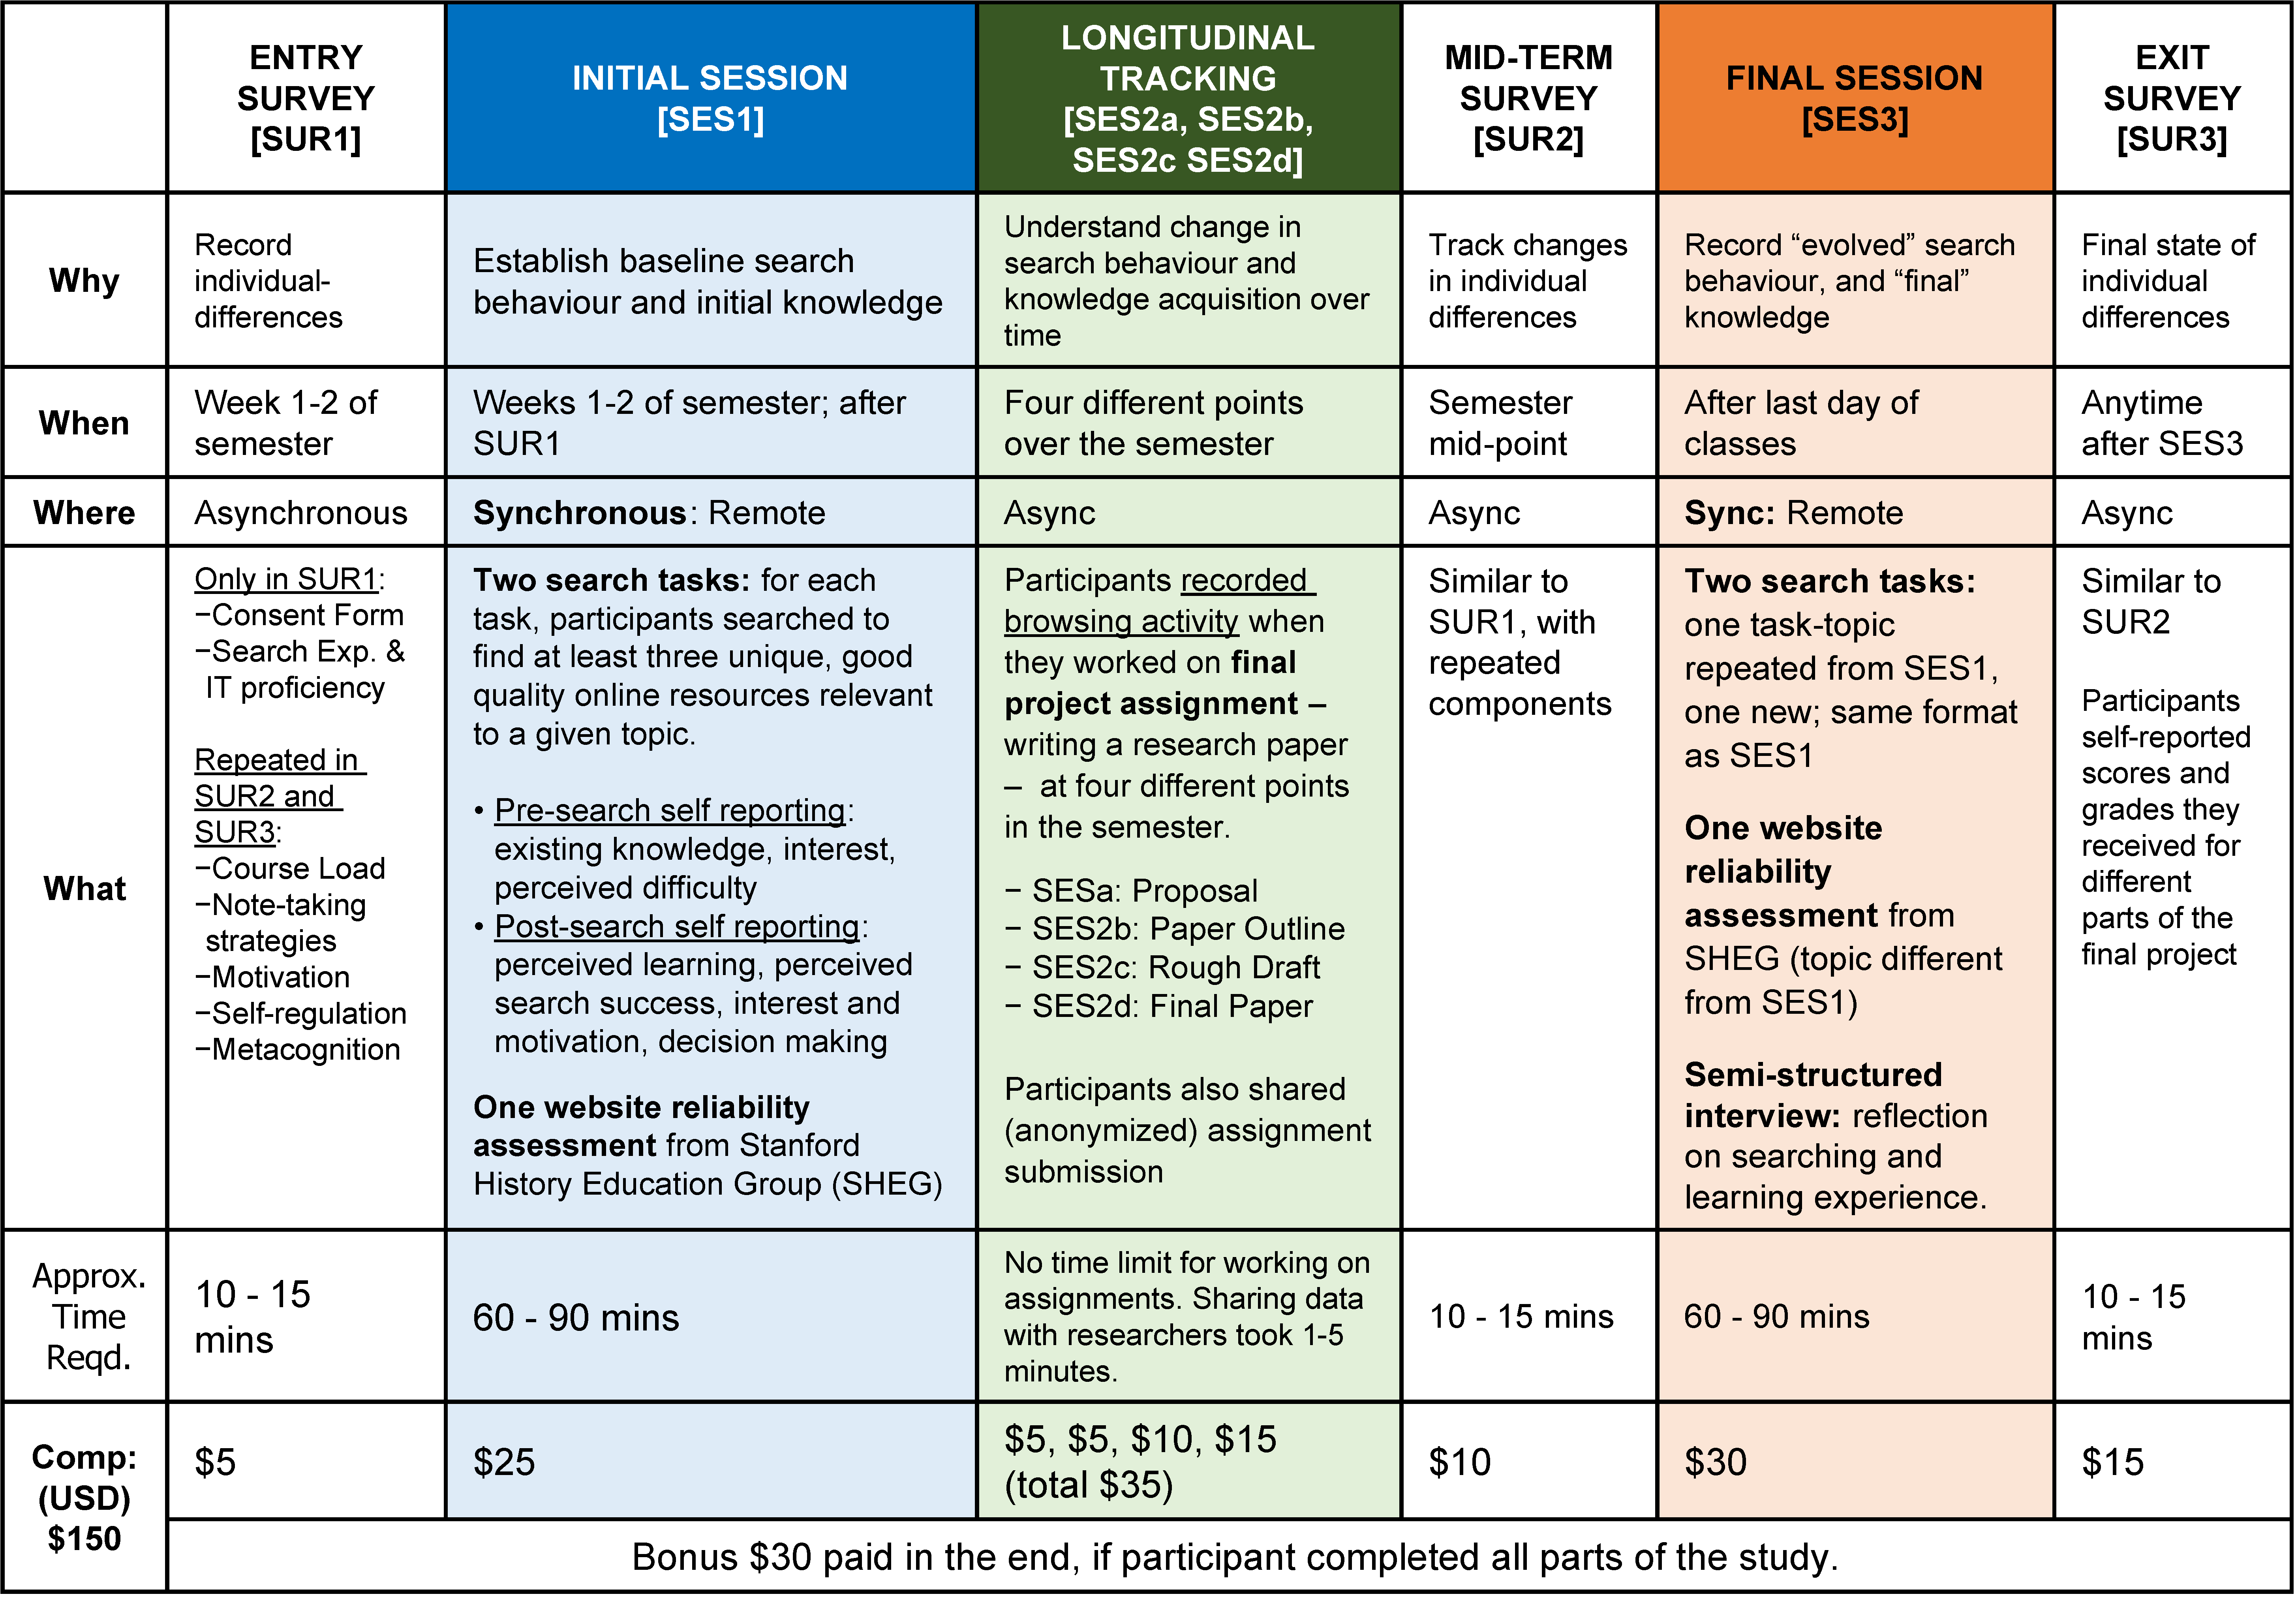
\includegraphics[width=1\linewidth]{figs/fig-study-proc-diss} 

}

\caption[Short Caption for LoF]{Very very very very very very very very long caption.}\label{fig:fig-study-proc-diss}
\end{figure}

Reference it

\hypertarget{sec-method-sur1}{%
\subsection{SUR1: Entry Survey}\label{sec-method-sur1}}

\hypertarget{ses1-initial-session}{%
\subsection{SES1: Initial Session}\label{ses1-initial-session}}

\hypertarget{ses2a---ses2d-longitudinal-tracking-sessions}{%
\subsection{SES2a - SES2d: Longitudinal Tracking Sessions}\label{ses2a---ses2d-longitudinal-tracking-sessions}}

\hypertarget{sec-method-sur2}{%
\subsection{SUR2: Mid-Term Survey}\label{sec-method-sur2}}

\hypertarget{ses3-final-session}{%
\subsection{SES3: Final Session}\label{ses3-final-session}}

\hypertarget{sur3-exit-survey}{%
\subsection{SUR3: Exit Survey}\label{sur3-exit-survey}}

\hypertarget{data-analysis}{%
\chapter{Data Analysis}\label{data-analysis}}

Note about pronouns:
all participants are referred to using gender-neutral they/them pronouns.

Final feedback:
P022Pisa said
\textgreater{} \emph{It is great to be able to participate in the research this semester. Using the extension somehow brings me postive feedback and that helps me in study I303. So I wanna say thank you}\\
\textgreater{} - P022Pisa

\hypertarget{data-cleaning-and-processing}{%
\section{Data Cleaning and Processing}\label{data-cleaning-and-processing}}

\hypertarget{data-analysis-approach}{%
\section{Data Analysis Approach}\label{data-analysis-approach}}

see crescenzi thesis

\hypertarget{url-categorization}{%
\section{URL Categorization}\label{url-categorization}}

\hypertarget{latent-profile-analysis}{%
\section{Latent Profile Analysis}\label{latent-profile-analysis}}

\hypertarget{dwell-time-analysis}{%
\section{Dwell Time Analysis}\label{dwell-time-analysis}}

\hypertarget{results}{%
\chapter{Results}\label{results}}

Also see Yung Sheng's Dissertation

\hypertarget{rq1---search-behaviours}{%
\section{RQ1: - search behaviours?}\label{rq1---search-behaviours}}

\hypertarget{q---query-reformulation}{%
\subsection{Q - query reformulation}\label{q---query-reformulation}}

\hypertarget{l---source-selection}{%
\subsection{L - source selection}\label{l---source-selection}}

\hypertarget{i---interacting-with-sources}{%
\subsection{I - interacting with sources}\label{i---interacting-with-sources}}

\hypertarget{rq2-mention-here}{%
\section{RQ2: mention here}\label{rq2-mention-here}}

\hypertarget{rq3-mention-here}{%
\section{RQ3: mention here}\label{rq3-mention-here}}

\hypertarget{rq4-mention-here}{%
\section{RQ4: mention here}\label{rq4-mention-here}}

\hypertarget{conclusions-contributions-and-future-work}{%
\chapter{Conclusions, Contributions, and Future Work}\label{conclusions-contributions-and-future-work}}

see Jacek's thesis

\hypertarget{research-summary}{%
\section{Research Summary}\label{research-summary}}

\hypertarget{summary-of-results}{%
\section{Summary of Results}\label{summary-of-results}}

\hypertarget{methodology}{%
\section{Methodology}\label{methodology}}

\hypertarget{contributions}{%
\section{Contributions}\label{contributions}}

\hypertarget{limitations}{%
\section{Limitations}\label{limitations}}

\begin{itemize}
\tightlist
\item
  No PDF
\item
  N=16 to N=10
\item
  Also check anticipated limitations section from proposal
\end{itemize}

\hypertarget{future-work}{%
\section{Future Work}\label{future-work}}

\startappendices

\hypertarget{ch_pilot_study}{%
\chapter{Prior Work: Pilot Study}\label{ch_pilot_study}}

\hypertarget{ses1-initial-session-1}{%
\section{SES1: Initial Session}\label{ses1-initial-session-1}}

\hypertarget{app_signup_survey}{%
\chapter{SUR1: Entry Survey}\label{app_signup_survey}}

\hypertarget{app_pre_post_tasks}{%
\chapter{Questionnaires for Initial (SES1) and Final (SES3) Sessions}\label{app_pre_post_tasks}}

\hypertarget{app_midterm_survey}{%
\chapter{SUR2: Midterm Survey}\label{app_midterm_survey}}

\hypertarget{app_final_survey}{%
\chapter{SUR3: Exit Survey}\label{app_final_survey}}

\hypertarget{app_variables}{%
\chapter{Variables and Measures}\label{app_variables}}

\hypertarget{sec_app_ack}{%
\chapter{Acknowledgements - The PhD Journey}\label{sec_app_ack}}

Similar to David Maxwell's thesis.

This section will be fleshed out in more detail after the initial committee-submission on Feb 27, 2023.
For now, I wish to thank the following people and organisations (in no particular order):

\begin{itemize}
\tightlist
\item
  Jacek Gwizdka
\item
  Soo Young Rieh + Funding
\item
  Committee Members
\item
  HEB
\item
  Finland people
\item
  Slovenia People
\item
  Germany People

  \begin{itemize}
  \tightlist
  \item
    Anke, Xiaofei, Michael, Hema, Himanshu, Ambika, Hardik\ldots{}
  \end{itemize}
\item
  India People
\item
  UK People
\item
  USA People
\item
  HCI4SouthAsia People
\item
  ASIST People
\item
  CHIIR People + Conferences
\item
  UT Graduate School Funding
\item
  SALPilot Study People
\item
  I303 People
\item
  DAAD
\item
  ABB
\item
  iSchool Doc Colleagues
\item
  Labmates, Officemates
\item
  LinkedIn people
\item
  Twitter people

  \begin{itemize}
  \tightlist
  \item
    Jason Baldridge
  \end{itemize}
\end{itemize}

\hypertarget{references}{%
\chapter*{References}\label{references}}
\addcontentsline{toc}{chapter}{References}

\markboth{References}{}

\hypertarget{refs}{}
\begin{CSLReferences}{1}{0}
\leavevmode\vadjust pre{\hypertarget{ref-agosti2014evaluation}{}}%
Agosti, M., Fuhr, N., Toms, E., \& Vakkari, P. (2014). Evaluation methodologies in information retrieval dagstuhl seminar 13441. \emph{ACM SIGIR Forum}, \emph{48}, 36--41.

\leavevmode\vadjust pre{\hypertarget{ref-allan2012frontiers}{}}%
Allan, J., Croft, B., Moffat, A., \& Sanderson, M. (2012). Frontiers, challenges, and opportunities for information retrieval: Report from SWIRL 2012 the second strategic workshop on information retrieval in lorne. \emph{ACM SIGIR Forum}, \emph{46}, 2--32.

\leavevmode\vadjust pre{\hypertarget{ref-ambrose2010howa}{}}%
Ambrose, S. A., Bridges, M. W., DiPietro, M., Lovett, M. C., \& Norman, M. K. (2010). \emph{How {Learning Works}: Seven {Research}-{Based Principles} for {Smart Teaching}}. {John Wiley \& Sons}.

\leavevmode\vadjust pre{\hypertarget{ref-amina2017active}{}}%
Amina, T. (2017). Active knowledge making: Epistemic dimensions of e-learning. In \emph{E-learning ecologies} (pp. 65--87). Routledge.

\leavevmode\vadjust pre{\hypertarget{ref-bhattacharya2021longitudinal}{}}%
Bhattacharya, N. (2021). A longitudinal study to understand learning during search. \emph{Proceedings of the 2021 Conference on Human Information Interaction and Retrieval}, 363--366.

\leavevmode\vadjust pre{\hypertarget{ref-borlund2013interactive}{}}%
Borlund, P. (2013). Interactive {Information Retrieval}: {An Introduction}. \emph{Journal of Information Science Theory and Practice}, \emph{1}(3), 12--32. \url{https://doi.org/10.1633/JISTAP.2013.1.3.2}

\leavevmode\vadjust pre{\hypertarget{ref-brookes1980foundations}{}}%
Brookes, B. C. (1980). The foundations of information science. Part i. Philosophical aspects. \emph{Journal of Information Science}, \emph{2}(3-4), 125--133.

\leavevmode\vadjust pre{\hypertarget{ref-collins2017search}{}}%
Collins-Thompson, K., Hansen, P., \& Hauff, C. (2017). Search as learning (dagstuhl seminar 17092). \emph{Dagstuhl Reports}, \emph{7}.

\leavevmode\vadjust pre{\hypertarget{ref-cope2017elearningc}{}}%
Cope, B., \& Kalantzis, M. (2017). \emph{E-{Learning Ecologies}: Principles for {New Learning} and {Assessment}}. {Taylor \& Francis}.

\leavevmode\vadjust pre{\hypertarget{ref-cope2013new}{}}%
Cope, B., \& Kalantzis, M. (2013). Towards a {New Learning}: The {\emph{Scholar}} {Social Knowledge Workspace}, in {Theory} and {Practice}. \emph{E-Learning and Digital Media}, \emph{10}(4), 332--356. \url{https://doi.org/10.2304/elea.2013.10.4.332}

\leavevmode\vadjust pre{\hypertarget{ref-eickhoff2017introduction}{}}%
Eickhoff, C., Gwizdka, J., Hauff, C., \& He, J. (2017). Introduction to the special issue on search as learning. \emph{Information Retrieval Journal}, \emph{20}(5), 399--402.

\leavevmode\vadjust pre{\hypertarget{ref-freund2013searching}{}}%
Freund, L., Gwizdka, J., Hansen, P., Kando, N., \& Rieh, S. Y. (2013). From searching to learning. \emph{Evaluation Methodologies in Information Retrieval. Dagstuhl Reports}, \emph{13441}, 102--105.

\leavevmode\vadjust pre{\hypertarget{ref-freund2014searching}{}}%
Freund, L., He, J., Gwizdka, J., Kando, N., Hansen, P., \& Rieh, S. Y. (2014). Searching as learning (SAL) workshop 2014. \emph{Proceedings of the 5th Information Interaction in Context Symposium}, 7--7.

\leavevmode\vadjust pre{\hypertarget{ref-gwizdka2016search}{}}%
Gwizdka, J., Hansen, P., Hauff, C., He, J., \& Kando, N. (2016). Search as learning (SAL) workshop 2016. \emph{Proceedings of the 39th International ACM SIGIR Conference on Research and Development in Information Retrieval}, 1249--1250.

\leavevmode\vadjust pre{\hypertarget{ref-hansen2016editorial}{}}%
Hansen, P., \& Rieh, S. Y. (2016). Editorial: Recent advances on searching as learning: An introduction to the special issue. \emph{Journal of Information Science}, \emph{42}(1), 3--6. \url{https://doi.org/10.1177/0165551515614473}

\leavevmode\vadjust pre{\hypertarget{ref-kalantzis2012newa}{}}%
Kalantzis, M., \& Cope, B. (2012). \emph{New {Learning}: Elements of a {Science} of {Education}}. {Cambridge University Press}.

\leavevmode\vadjust pre{\hypertarget{ref-karapanos2021advances}{}}%
Karapanos, E., Gerken, J., Kjeldskov, J., \& Skov, M. B. (Eds.). (2021). \emph{Advances in {Longitudinal HCI Research}}. {Springer International Publishing}. \url{https://doi.org/10.1007/978-3-030-67322-2}

\leavevmode\vadjust pre{\hypertarget{ref-kelly2006measuring_a}{}}%
Kelly, D. (2006a). Measuring online information seeking context, {Part} 1: Background and method. \emph{Journal of the American Society for Information Science and Technology}, \emph{57}(13), 1729--1739. \url{https://doi.org/10.1002/asi.20483}

\leavevmode\vadjust pre{\hypertarget{ref-kelly2006measuring_b}{}}%
Kelly, D. (2006b). Measuring online information seeking context, {Part} 2: Findings and discussion. \emph{Journal of the American Society for Information Science and Technology}, \emph{57}(14), 1862--1874. \url{https://doi.org/10.1002/asi.20484}

\leavevmode\vadjust pre{\hypertarget{ref-kelly2009evaluation}{}}%
Kelly, D., Dumais, S., \& Pedersen, J. O. (2009). Evaluation challenges and directions for information-seeking support systems. \emph{IEEE Computer}, \emph{42}(3).

\leavevmode\vadjust pre{\hypertarget{ref-ko2021seeking}{}}%
Ko, A. J. (2021). Seeking information. In \emph{Foundations of {Information}}. \url{https://faculty.washington.edu/ajko/books/foundations-of-information/\#/seeking}

\leavevmode\vadjust pre{\hypertarget{ref-HCIUXres81_online}{}}%
Koeman, L. (2020). \emph{HCI/UX research: What methods do we use? -- lisa koeman -- blog}. \url{https://lisakoeman.nl/blog/hci-ux-research-what-methods-do-we-use/}.

\leavevmode\vadjust pre{\hypertarget{ref-kuhlthau2004seeking}{}}%
Kuhlthau, C. C. (2004). \emph{Seeking meaning: A process approach to library and information services} (Vol. 2). Libraries Unlimited Westport, CT.

\leavevmode\vadjust pre{\hypertarget{ref-marchionini1995information}{}}%
Marchionini, G. (1995). \emph{Information {Seeking} in {Electronic Environments}}. {Cambridge University Press}.

\leavevmode\vadjust pre{\hypertarget{ref-marchionini2006toward}{}}%
Marchionini, G. (2006). Toward human-computer information retrieval. \emph{Bulletin of the American Society for Information Science and Technology}, \emph{32}(5), 20--22.

\leavevmode\vadjust pre{\hypertarget{ref-council2000how}{}}%
National Research Council. (2000). \emph{How people learn: {Brain}, mind, experience, and school: {Expanded} edition}. {The National Academies Press}. \url{https://doi.org/10.17226/9853}

\leavevmode\vadjust pre{\hypertarget{ref-newlondon1996pedagogy}{}}%
New London Group. (1996). A pedagogy of multiliteracies: Designing social futures. \emph{Harvard Educational Review}, \emph{66}(1), 60--92.

\leavevmode\vadjust pre{\hypertarget{ref-novak2010learninga}{}}%
Novak, J. D. (2010). \emph{Learning, creating, and using knowledge: Concept maps as facilitative tools in schools and corporations} (2nd ed). {Routledge}.

\leavevmode\vadjust pre{\hypertarget{ref-url_rieh_homepage}{}}%
Rieh, S. Y. (2020). \emph{Research area 1: Searching as learning}. \url{https://rieh.ischool.utexas.edu/research}.

\leavevmode\vadjust pre{\hypertarget{ref-rieh2016searching}{}}%
Rieh, S. Y., Collins-Thompson, K., Hansen, P., \& Lee, H.-J. (2016). Towards searching as a learning process: A review of current perspectives and future directions. \emph{Journal of Information Science}, \emph{42}(1), 19--34. \url{https://doi.org/10.1177/0165551515615841}

\leavevmode\vadjust pre{\hypertarget{ref-sawyer2005cambridge}{}}%
Sawyer, R. K. (2005). \emph{The {Cambridge} handbook of the learning sciences}. {Cambridge University Press}.

\leavevmode\vadjust pre{\hypertarget{ref-vakkari2016searching}{}}%
Vakkari, P. (2016). Searching as learning: A systematization based on literature. \emph{Journal of Information Science}, \emph{42}(1), 7--18. \url{https://doi.org/10.1177/0165551515615833}

\leavevmode\vadjust pre{\hypertarget{ref-vakkari2001changes}{}}%
Vakkari, P. (2001). Changes in search tactics and relevance judgements when preparing a research proposal a summary of the findings of a longitudinal study. \emph{Information Retrieval}, \emph{4}(3), 295--310.

\leavevmode\vadjust pre{\hypertarget{ref-weber2019informationseeking}{}}%
Weber, H., Becker, D., \& Hillmert, S. (2019). Information-seeking behaviour and academic success in higher education: Which search strategies matter for grade differences among university students and how does this relevance differ by field of study? \emph{Higher Education}, \emph{77}(4), 657--678. \url{https://doi.org/10.1007/s10734-018-0296-4}

\leavevmode\vadjust pre{\hypertarget{ref-weber2018can}{}}%
Weber, H., Hillmert, S., \& Rott, K. J. (2018). Can digital information literacy among undergraduates be improved? Evidence from an experimental study. \emph{Teaching in Higher Education}, \emph{23}(8), 909--926. \url{https://doi.org/10.1080/13562517.2018.1449740}

\leavevmode\vadjust pre{\hypertarget{ref-white2016interactions}{}}%
White, R. (2016a). \emph{Interactions with search systems}. Cambridge University Press.

\leavevmode\vadjust pre{\hypertarget{ref-white_2016_iwss_learning}{}}%
White, R. (2016b). Learning and use. In \emph{Interactions with search systems} (pp. 231--248). {Cambridge University Press}. \url{https://doi.org/10.1017/CBO9781139525305.010}

\leavevmode\vadjust pre{\hypertarget{ref-white2009characterizing}{}}%
White, R., Dumais, S., \& Teevan, J. (2009). Characterizing the influence of domain expertise on web search behavior. \emph{Proceedings of the {Second ACM International Conference} on {Web Search} and {Data Mining} - {WSDM} '09}, 132. \url{https://doi.org/10.1145/1498759.1498819}

\leavevmode\vadjust pre{\hypertarget{ref-wildemuth2004effects}{}}%
Wildemuth, B. M. (2004). The effects of domain knowledge on search tactic formulation. \emph{Journal of the American Society for Information Science and Technology}, \emph{55}(3), 246--258. \url{https://doi.org/10.1002/asi.10367}

\leavevmode\vadjust pre{\hypertarget{ref-zlatkin2021students}{}}%
Zlatkin-Troitschanskaia, O., Hartig, J., Goldhammer, F., \& Krstev, J. (2021). Students' online information use and learning progress in higher education \textendash{} {A} critical literature review. \emph{Studies in Higher Education}, 1--26. \url{https://doi.org/10.1080/03075079.2021.1953336}

\end{CSLReferences}

%%%%% REFERENCES


\end{document}
